% --------------------------------------------------------------
% This is all preamble stuff that you don't have to worry about.
% Head down to where it says "Start here"
% --------------------------------------------------------------

\title{Classification de places de parking}
\author{Lionel Cheng}
\date{Juin 2022}

\documentclass[12pt]{article}

% Math
\usepackage{amsmath,amsthm,amssymb}
\usepackage{stmaryrd}

% Physics
\usepackage{physics}
\usepackage[version=4]{mhchem}
\usepackage{chemist}
\usepackage{siunitx}

% Other
\usepackage[margin=1in]{geometry}
\usepackage[utf8]{inputenc}
\usepackage[T1]{fontenc}
\usepackage{graphicx}
\usepackage{longtable}
\usepackage{array}
\usepackage{empheq}
\usepackage{enumitem}
\usepackage{scalerel}
\usepackage{subcaption}

% For bold upgreek letters
\usepackage{upgreek}
\usepackage{stmaryrd}
\SetSymbolFont{stmry}{bold}{U}{stmry}{m}{n}
\usepackage{bm}

% Bibliography
\usepackage{natbib}

\usepackage{xcolor}
\definecolor{linkcol}{rgb}{0,0,0.4}
\definecolor{citecol}{rgb}{0.5,0,0}
\definecolor{blue_sketch}{rgb}{0,0,0.4}
\definecolor{red_sketch}{rgb}{0.5,0,0}
\usepackage{hyperref}
\hypersetup{
    colorlinks=true,
    citecolor=citecol,
    linkcolor=linkcol,
    urlcolor=linkcol,
    linktoc=all
}

\newtheorem{definition}{Definition}[section]
\newtheorem{property}{Property}[section]
\newtheorem{theorem}{Theorem}[section]

% TikZ
\usepackage{tikz}
\usetikzlibrary{shapes.geometric, arrows}
\usetikzlibrary{calc}
\usepackage{algorithm2e}

\usepackage[printonlyused,nohyperlinks]{acronym}

%%%% Confusion Matrix Body %%%%
\newcommand\MyBox[1]{%
    \fbox{\parbox[c][3cm][c]{3cm}{\centering #1}}%
    % Size of boxes
}
\newcommand\MyVBox[1]{%
    \parbox[c][1cm][c]{1cm}{\centering\bfseries #1}%
}
\newcommand\MyHBox[2][\dimexpr3cm+2\fboxsep\relax]{%
    \parbox[c][1cm][c]{#1}{\centering\bfseries #2}%
}
\newcommand\MyTBox[4]{%
    \MyVBox{#1}
    \MyBox{#2}\hspace*{-\fboxrule}%
    \MyBox{#3}\par\vspace{-\fboxrule}%
}
%%%%
\newcommand*\rot{\rotatebox{90}}

% Commands related to ensembles
\newcommand{\N}{\mathbb{N}}
\newcommand{\Z}{\mathbb{Z}}
\newcommand{\R}{\mathbb{R}}
\newcommand{\C}{\mathbb{C}}
\newcommand{\Ltwo}[1]{\mathcal{L}^2(#1)}

% Intervals
\newcommand{\intint}[2]{\llbracket #1, #2 \rrbracket}

% Vectors/Tensors and bold symbols
\newcommand{\ve}[1]{\vb*{#1}}
\newcommand{\x}{\vb{x}}
\newcommand{\vr}{\vb{r}}
\newcommand{\vv}{\vb{v}}
\newcommand{\kv}{\vb{k}}
\newcommand{\av}{\vb{a}}
\newcommand{\U}{\vb{U}}
\newcommand{\uv}{\vb{u}}
\newcommand{\er}{\vb{e}_r}
\newcommand{\et}{\vb{e}_\theta}
\newcommand{\vt}{\vb{t}}
\newcommand{\vF}{\vb{F}}
\newcommand{\ex}{\vb{e}_x}

% Derivatives
\newcommand{\dtadv}[2]{\frac{\delta #1}{\delta #2}}
\newcommand{\ut}{\pdv{u}{t}}
\newcommand{\ux}{\pdv{u}{x}}
\newcommand{\uxx}{\pdv[2]{u}{x}}

% Operators
\newcommand{\hf}{\hat{f}}
\newcommand{\hu}{\hat{u}}
\newcommand{\e}{\mathrm{e}}
\newcommand{\ii}{\mathrm{i}}
\newcommand{\F}{\mathcal{F}}
\newcommand{\I}{\mathrm{I}}

% Capital greek letters not in italic (delta and omega)
\DeclareMathSymbol{\upD}{\mathalpha}{operators}{1}
\DeclareMathSymbol{\upP}{\mathalpha}{operators}{5}
\DeclareMathSymbol{\upS}{\mathalpha}{operators}{6}
\DeclareMathSymbol{\upO}{\mathalpha}{operators}{10}
\newcommand{\dt}{\upD t}
\newcommand{\dx}{\upD x}
\newcommand{\dy}{\upD y}
\newcommand{\lapl}{\upD}

% Finite element
\newcommand{\sumfe}{\sum_{\tau \in E(i)} \sum_{k \in \tau}}
\newcommand{\sumcell}{\sum_{\tau \in E(i)}}

% Redefinition (more compact)
\newcommand{\veps}{\varepsilon}
\newcommand{\eps}{\epsilon}
\newcommand{\psc}{\scaleto{\partial}{5pt}}
\newcommand{\mrm}{\mathrm}
\newcommand{\mc}{\mathcal}
\newcommand{\ta}{\theta}
\newcommand{\tij}{t_{ij}}
\newcommand{\phij}{\phi_{i, j}}
\newcommand{\tS}{\tilde{S}}
\newcommand{\tN}{\tilde{N}}
\newcommand{\tR}{\tilde{R}}
\newcommand{\tin}{\mathrm{in}}
\newcommand{\out}{\mathrm{out}}

% Misc (rather long formulas)
\newcommand{\green}{G(\vb{x}, \vb{x}')}
\newcommand{\cylgrad}[3]{\dfrac{\partial #1}{\partial r} + \dfrac{1}{r} \dfrac{\partial #2}{\partial \theta} + \dfrac{\partial #3}{\partial z}}
\newcommand{\cyldiv}[3]{\dfrac{1}{r}\dfrac{\partial r #1}{\partial r} + \dfrac{1}{r} \dfrac{\partial #2}{\partial \theta} + \dfrac{\partial #3}{\partial z}}

% Quantum mechanics
\newcommand{\mean}[1]{\langle #1 \rangle}
\newcommand{\wf}{\psi(\ve{r}, t)}
\newcommand{\ham}{\hat{H}}
\newcommand{\hA}{\hat{A}}
\newcommand{\hB}{\hat{B}}
\newcommand{\upd}{\mathrm{d}}
\newcommand{\psia}{\psi_\alpha(\ve{r})}
\newcommand{\kpsi}{\ket{\psi}}
\newcommand{\bpsi}{\bra{\psi}}
\newcommand{\kb}{\ket{n}}
\newcommand{\knr}{\ket{n, r}}
\newcommand{\kpsiz}{\ket{\psi^0}}
\newcommand{\kpsio}{\ket{\psi^1}}
\newcommand{\kpsit}{\ket{\psi^2}}
\newcommand{\hv}[1]{\hat{\vb*{#1}}}
\newcommand{\hvr}{\hat{\vb{r}}}
\newcommand{\vp}{\vb*{p}}
\newcommand{\hvp}{\hat{\vb*{p}}}
\newcommand{\kpsin}{\ket{\psi_n}}
\newcommand{\bpsin}{\bra{\psi_n}}
\newcommand{\hO}{\hat{O}}

% Statistical Physics and kinetic theory
\newcommand{\Ni}{\mathcal{N}_i}
\newcommand{\NN}{\mathcal{N}}
\newcommand{\Qrot}{\mathcal{Q}^\text{rot}}
\newcommand{\Q}{\mathcal{Q}}
\newcommand{\evibsnv}{\epsilon_\text{s,nv}^\text{vib}}
\newcommand{\erotsnv}{\epsilon_\text{s,nv}^\text{rot}}
\newcommand{\evib}{\varepsilon_\text{vib}}
\newcommand{\eR}{\varepsilon_R}
\newcommand{\fastp}{\dot{E}^p_\text{fast}}
\newcommand{\vibp}{\dot{E}^p_\text{vib}}
\newcommand{\vfone}{\vb{f}_{1}}
\newcommand{\di}{\mathrm{d}}
\newcommand{\tA}{\mathrm{A}}
\newcommand{\tBC}{\mathrm{BC}}
\newcommand{\vib}{\text{vib}}
\newcommand{\Ntwo}{\ce{N2}}
\newcommand{\Otwo}{\ce{O2}}
\newcommand{\qlpl}{\{q_l, p_l\}}
\newcommand{\dqdp}{\prod_l dq_l dp_l}

% Relaxation times
\newcommand{\tautt}{\tau_\text{TT}}
\newcommand{\taurt}{\tau_\text{RT}}
\newcommand{\tauvt}{\tau_\text{VT}}
\newcommand{\Erot}{E_\text{rot}}
\newcommand{\Evib}{E_\text{vib}}

% Metric related properties
\newcommand{\dvi}{\partial V_i}
\newcommand{\Sij}{\vb{S}_{i, j}^\tau}
\newcommand{\Si}{\vb{S}_i^\tau}
\newcommand{\pipe}[1]{\left. #1 \right\vert}

% Units
\newcommand{\ns}{\SI{}{\nano\second}}
\newcommand{\mus}{\SI{}{\micro\second}}
\newcommand{\ms}{\SI{}{\milli\second}}
\newcommand{\kHz}{\SI{}{\kilo\hertz}}

% Small partial in integrals
\newcommand\ppartial{\scaleobj{0.7}{\partial}}

% Differential
\newcommand{\md}{\mrm{d}}

% Environnement pour insérer une image en dehors des marges - bigcenter
\makeatletter
\newskip\@bigflushglue \@bigflushglue = -200pt plus 1fil
\def\bigcenter{\trivlist \bigcentering\item\relax}
\def\bigcentering{\let\\\@centercr\rightskip\@bigflushglue%
	\leftskip\@bigflushglue
	\parindent\z@\parfillskip\z@skip}
\def\endbigcenter{\endtrivlist}

\newcommand\highlight[1]{{\textcolor{red}{#1}}}


% Theorems and definitions

\begin{document}
\maketitle

% --------------------------------------------------------------
%                         Start here
% --------------------------------------------------------------

\section{Contexte et présentation du problème}

L'objectif de ce travail est de proposer une méthodologie et de répondre à des questions autour de la détection automatique en temps réel de l'occupation de places de parking par traitement d'images. La méthode doit pouvoir être implémentable sur un nano-ordinateur de type Raspberry Pi. Deux étapes sont nécessaires pour répondre à ce problème:

\begin{itemize}
    \item La détection des places de parking à partir de la vidéo d'une caméra
    \item L'occupation de chaque place
\end{itemize}

Ce document se focalise sur la deuxième étape de ce problème, la première pouvant être traitée par un Mask R-CNN \citep{He2017} ou alors en segmentant directement la caméra que l'on utilise en délimitant les places, les caméras de surveillance de parking étant immobiles la plupart du temps.

Nous avons donc affaire à une tâche de classification d'images à 2 classes: occupée ou libre. Des réseaux de neurones vont être utilisés pour répondre à ce problème, ceux-ci étant particulièrement rapides et efficaces pour le traitment d'images depuis l'avènement d'AlexNet \citep{alexnet}.

\section{Données}

Le jeu de données suggéré dans l'énoncé, PKLot, a été publié en 2015 \citep{deAlmeida2015} et est le premier jeu de données aussi conséquent d'images de parkings. Celui-ci contient 12416 images de parkings provenant de 3 cameras de surveillance (PUC, UFPR04 et UFPR05) prises à différents moments de la journée sur plusieurs jours. Ces images sont segmentées en 695 899 images de places de parking individuelles \citep{deAlmeida2015}. Celles-ci ont des orientations et des éclairages différents en fonction de la météo. On peut voir des images complètes des 3 caméras en Fig.~\ref{fig:pklot_video_feed} et des images segmentées en Fig.~\ref{fig:pklot_individual}.

\begin{figure}[htbp]
    \centering
    \begin{subfigure}{0.7\textwidth}
        \centering
        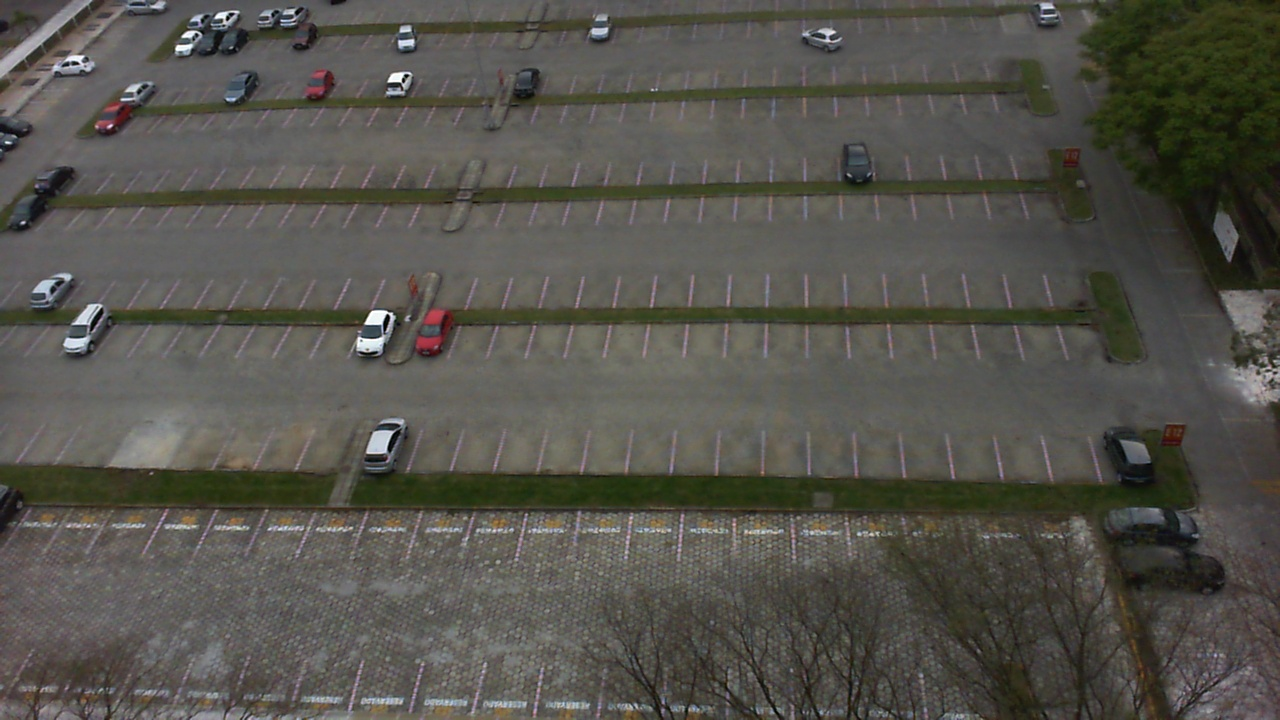
\includegraphics[width=\textwidth]{figures/datasets/2012-09-12_07_02_42.jpg}
        \caption{Caméra PUC}
    \end{subfigure}
    \begin{subfigure}{0.45\textwidth}
        \centering
        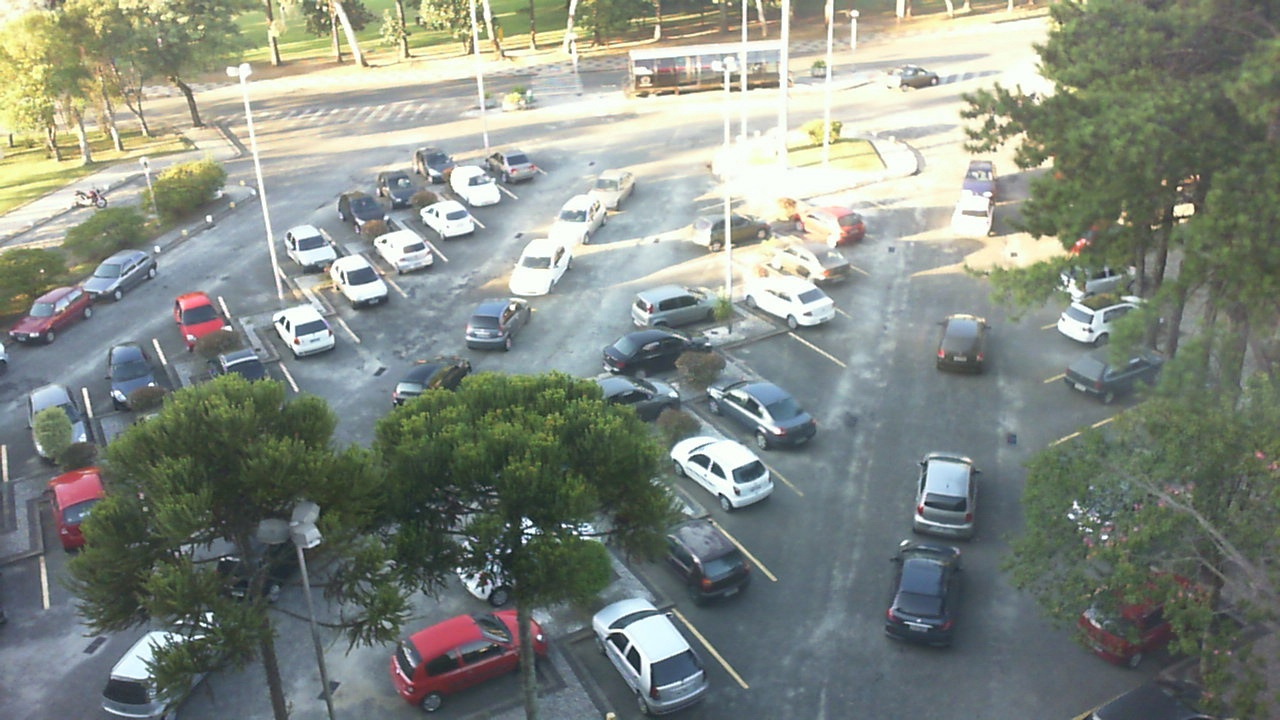
\includegraphics[width=\textwidth]{figures/datasets/2013-01-29_20_21_23.jpg}
        \caption{Caméra UFPR04}
    \end{subfigure}
    \begin{subfigure}{0.45\textwidth}
        \centering
        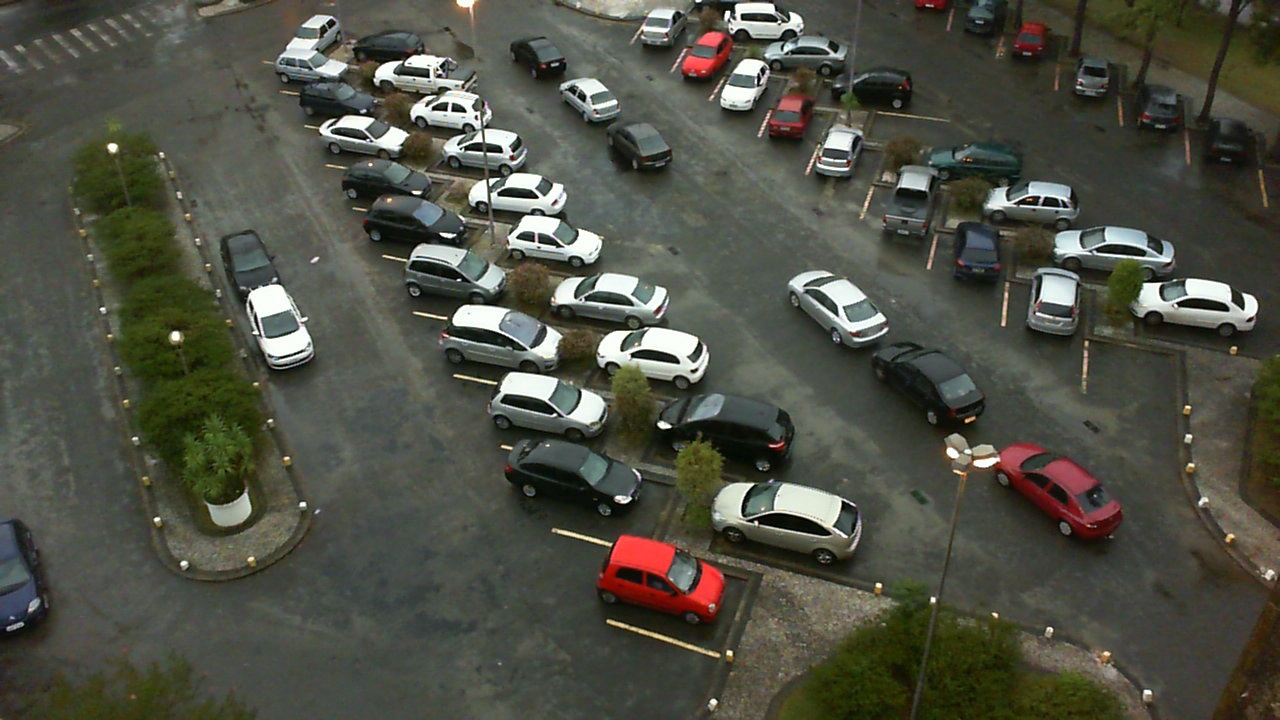
\includegraphics[width=\textwidth]{figures/datasets/2013-04-12_16_20_11.jpg}
        \caption{Caméra UFPR05}
    \end{subfigure}
    \caption{Vue complète des caméras de surveillance du jeu de données PKLot.}
    \label{fig:pklot_video_feed}
\end{figure}

\begin{figure}[htbp]
    \centering
    \begin{subfigure}{0.2\textwidth}
        \centering
        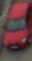
\includegraphics[width=\textwidth]{figures/datasets/2012-09-12_07_02_42_050.jpg}
        \caption{Occupée}
    \end{subfigure}
    \begin{subfigure}{0.2\textwidth}
        \centering
        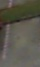
\includegraphics[width=\textwidth]{figures/datasets/2012-09-12_07_02_42_051.jpg}
        \caption{Libre}
    \end{subfigure}
    \begin{subfigure}{0.2\textwidth}
        \centering
        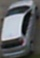
\includegraphics[width=\textwidth]{figures/datasets/2012-09-12_07_02_42_072.jpg}
        \caption{Occupée}
    \end{subfigure}
    \begin{subfigure}{0.2\textwidth}
        \centering
        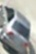
\includegraphics[width=\textwidth]{figures/datasets/2013-01-29_18_46_21_021.jpg}
        \caption{Occupée}
    \end{subfigure}
    \caption{Images de places de parkings labellisées provenant du jeu de données PKLot.}
    \label{fig:pklot_individual}
\end{figure}

Il y a environ 350 000 images par classe dans le jeu de données PKLot. Ce nombre semble largement suffisant lorsqu'on le compare à d'autres jeux de données d'images classiques tels que ImageNet LSVRC-2010 \citep{ILSVRC15} (1200 images par classe en moyenne), MNIST \citep{deng2012mnist} (700 images par classe), CIFAR-10 et CIFAR-100 \citep{Krizhevsky09learningmultiple} (6000 et 600 images par classe respectivement).

Plus que la taille du jeu de données, sa qualité doit être un critère primordial pour entraîner un réseau de neurones. Si celui-ci est trop biaisé dans un sens (une seule position de voiture par exemple) ou si les exemples sont trop simples, le réseau aura du mal à généraliser ses résultats.

Lorsque la taille du dataset n'est pas assez conséquente plusieurs techniques s'offrent à nous pour faire de \textbf{l'augmentation de données}. Ces opérations permettent d'éviter le sur-apprentissage (ou \textit{over-fitting} en anglais).

Une manière évidente est de réaliser des opérations sur le dataset existant tels que tourner, flouter, redimensionner ou encore contraster les images. Ces opérations sont illustrés en Fig.~\ref{fig:data_augmentation}.

\begin{figure}[htbp]
    \centering
    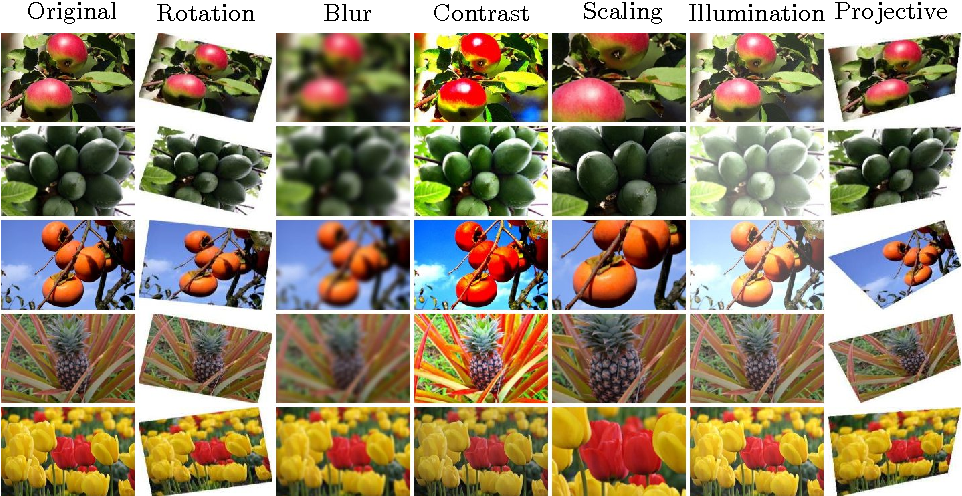
\includegraphics[width=0.8\textwidth]{figures/datasets/dataaugmention_illustration.png}
    \caption{Méthodes d'augmentation de données par modification du dataset existant.}
    \label{fig:data_augmentation}
\end{figure}

Des techniques plus avancées peuvent être utilisées tels que la génération d'images par GAN (Generative Adverserial Network) comme par exemple en utilisant le CycleGAN de \cite{CycleGAN2017}. Des illustrations des capacités du CycleGAN sont montrées en Fig.~\ref{fig:data_augmentation_gan}.

\begin{figure}[htbp]
    \centering
    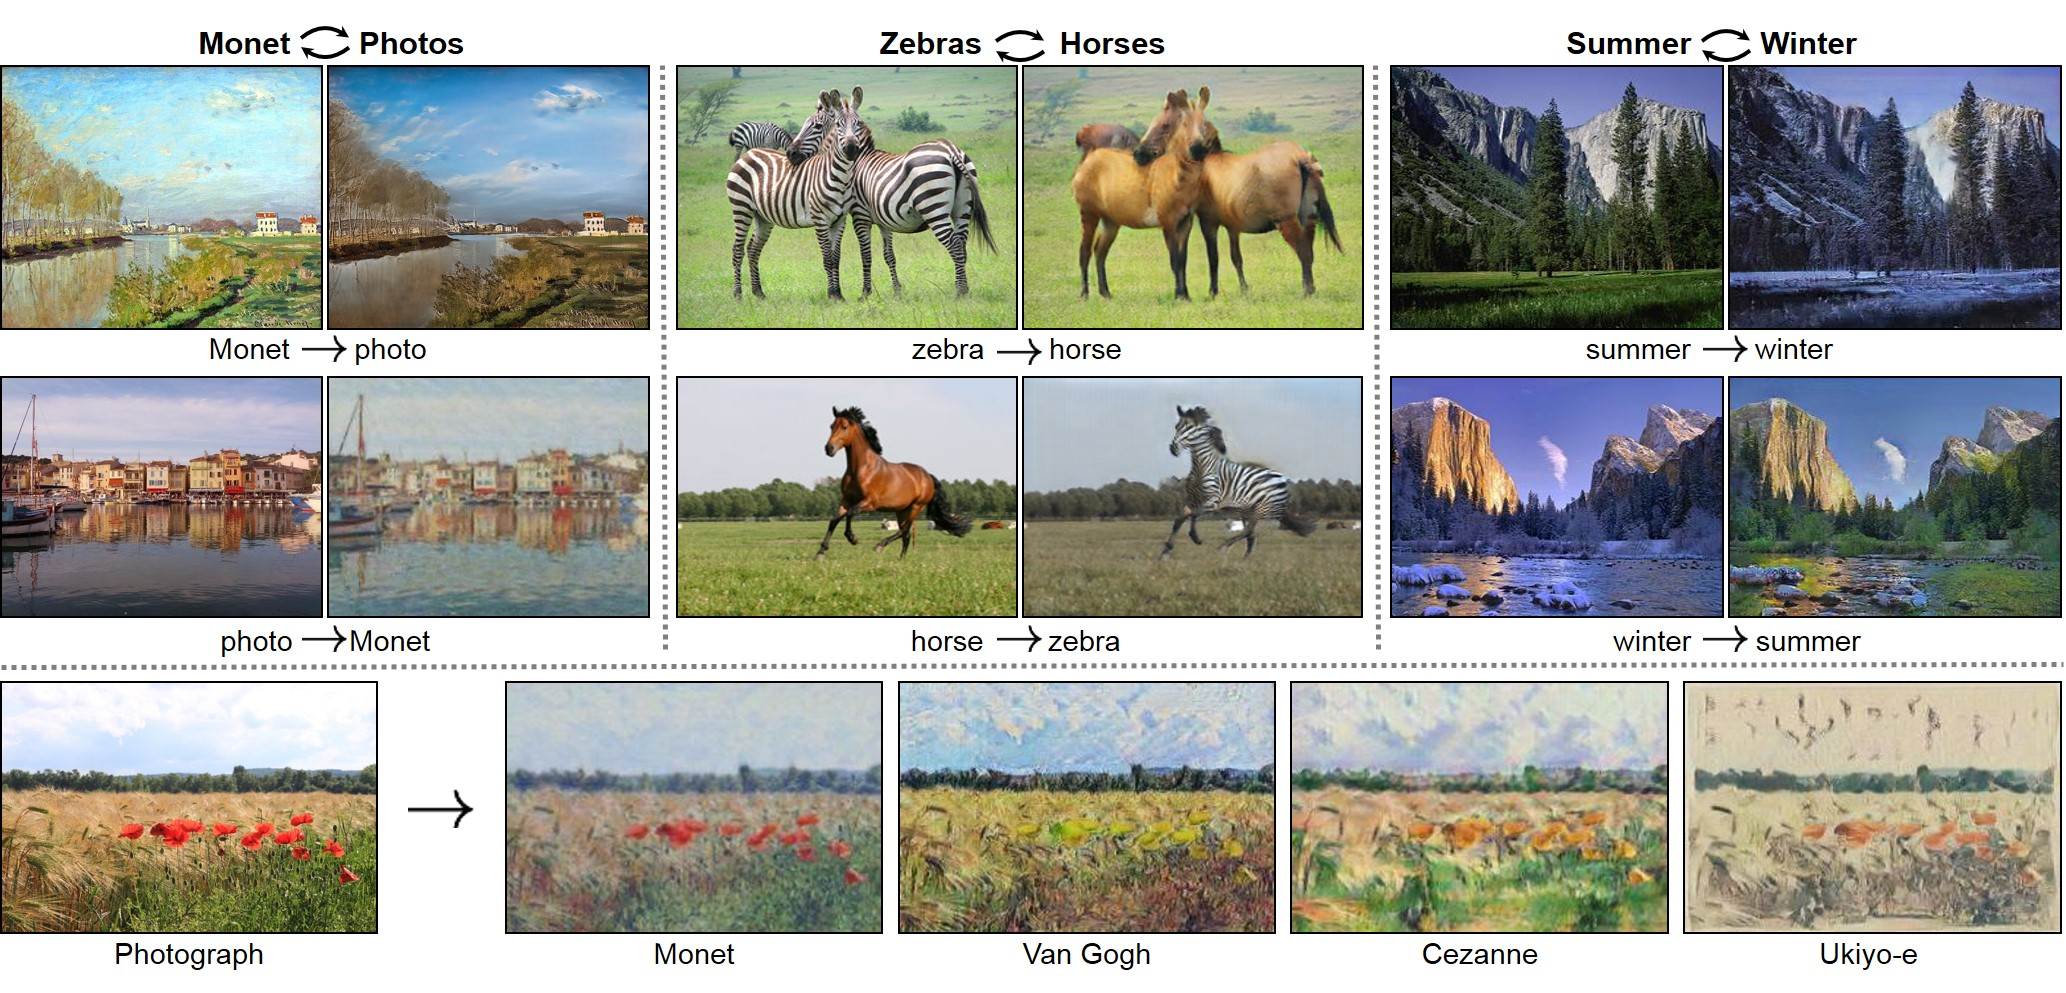
\includegraphics[width=\textwidth]{figures/datasets/cycle_gan.jpg}
    \caption{Méthodes d'augmentation de données par génération d'images synthétiques en utilisant le CycleGAN \citep{CycleGAN2017}.}
    \label{fig:data_augmentation_gan}
\end{figure}

\section{Modélisation}

Face à cette tâche de classification d'images, nous nous orientons vers des réseaux de neurones profonds convolutionnels (\textit{deep CNN} en anglais pour Convolutional Neural Network). Ces méthodes sont en effet les meilleurs pour les tâches de classification d'images depuis l'avènement d'AlexNet \citep{alexnet}, le premier réseau de neurones à avoir remporté avec beaucoup de marge la compétition ImageNet Large Scale Visual Recognition Challenge en 2012, mentionné en première partie de ce document. L'architecture du réseau est montrée en Fig.~\ref{fig:alexnet}.

\begin{figure}[htbp]
    \centering
    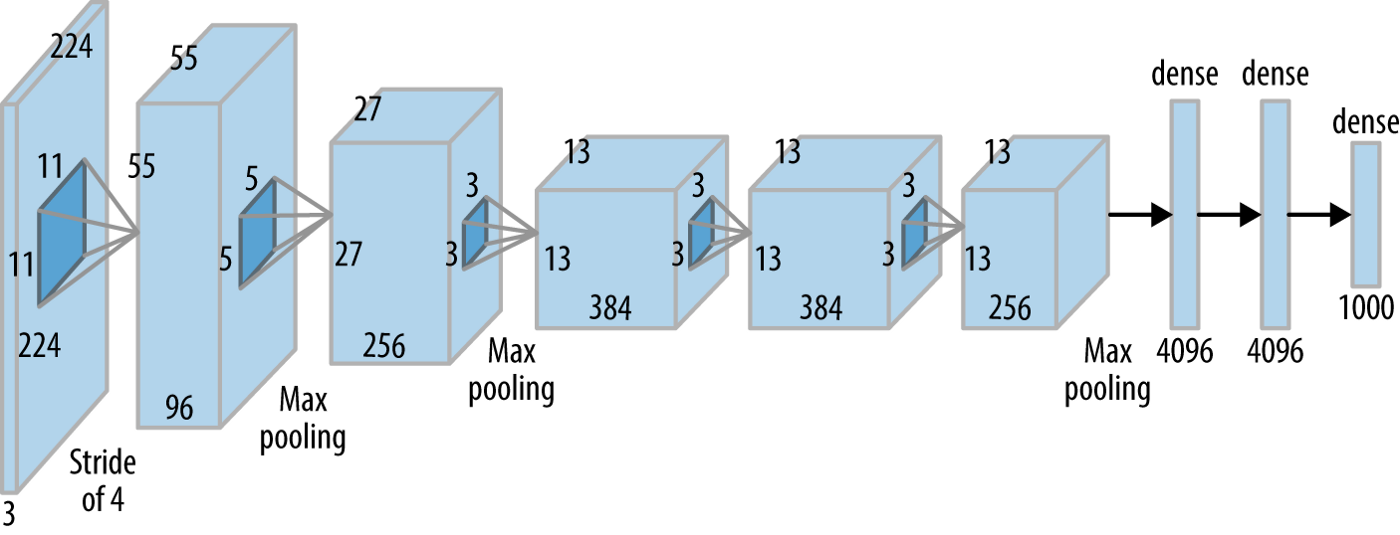
\includegraphics[width=0.8\textwidth]{figures/networks/alexnet.png}
    \caption{L'architecture d'AlexNet \citep{alexnet}.}
    \label{fig:alexnet}
\end{figure}

AlexNet contient environ 60 million de paramètres pour classifier 1000 différents familles d'images. Par rapport à notre tâche de classification binaire, on peut penser que son architecture est bien trop volumineuse et qu'un réseau plus petit sera à même d'être performant pour notre tâche de classification de places occupées ou libres. C'est justement ce qui est fait dans \citep{Amato2017} où une version allégée d'AlexNet qui contient plus de 1000 fois moins de paramètres est crée sous le nom de mAlexNet. L'architecture de ce réseau réduit est montrée en Fig.~\ref{fig:malexnet}.

\begin{figure}[htbp]
    \centering
    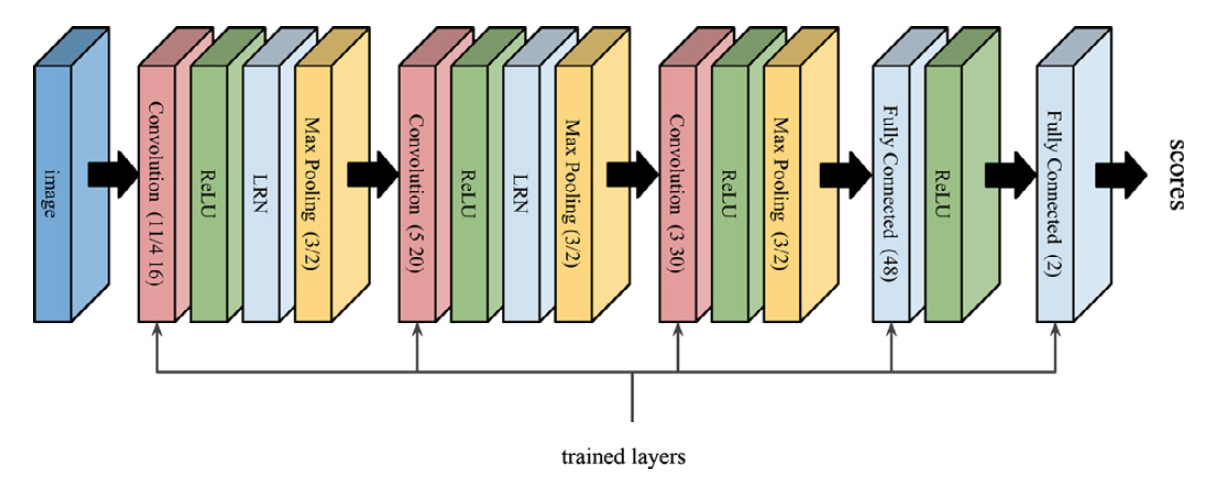
\includegraphics[width=0.7\textwidth]{figures/networks/malexnet.png}
    \caption{L'architecture de mAlexNet \citep{Amato2017}.}
    \label{fig:malexnet}
\end{figure}

En terms de CNNs plus légers et adaptés à notre cas on peut penser aux CNNs travaillant sur le jeu de données MNIST, des images de chiffres en noir et blanc écrits à la main, qui est une tâche de classification comprenant 10 familles (les chiffres de 0 à 9). Le réseau le plus établi pour résoudre cette tâche est le CNN LeNet5 \citep{lecun1998} dont l'architecture est montrée en Fig.~\ref{fig:lenet5}.

\begin{figure}[htbp]
    \centering
    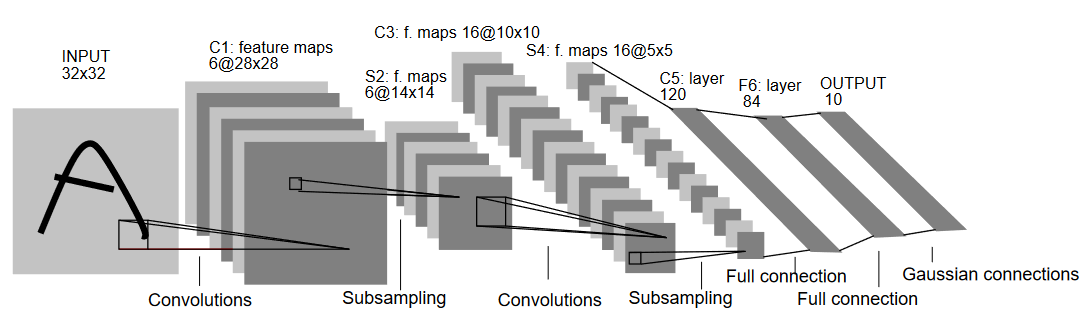
\includegraphics[width=0.8\textwidth]{figures/networks/lenet5.png}
    \caption{L'architecture de LeNet5 \citep{lecun1998}.}
    \label{fig:lenet5}
\end{figure}

Tous ces réseaux suivent une logique similaire: en partant de l'image pixellisée (avec un champ de couleur pour MNIST ou 3 pour les images de parking ou ImageNet), plusieurs couches de convolution/pooling sont appliquées avec des fonctions d'activation puis ces couches de convolution sont mises à plat (\textit{flatten} en anglais) et des couches de perceptrons (\textit{multi-layer perceptron} en anglais) sont ensuite appliquées. La dernière couche comprend autant de perceptrons que le nombre de classes et une opération de Softmax qui convertit ces amplitudes en probabilités est réalisée. La fonction de coût utilisée correspond alors à une entropie croisée (\textit{cross-entropy} en anglais):

\begin{equation}
    l(x, y) = \frac{1}{N} \sum_{n=1}^N l_n \qq{où} l_n = - \log \frac{\exp(x_{n, y_n})}{\sum_{c=1}^C \exp(x_{n,c})}
\end{equation}

\noindent où $N$ représente le batch-size et $x_{n, c}$ correspond à la dernière couche du réseau avant l'opération de Softmax qui est explicitée dans la fonction de coût ici.

Dans cette tâche de classification binaire, la métrique de performance la plus évident est l'exactitude (ou \textit{accuracy} que l'on dénote $\mrm{ACC}$) en anglais qui est la proportion de places correctemment classifiées sur le nombre de places total. Pour définir d'autres métriques et comprendre un peu plus le comportement du réseau on fait appel à la matrice de confusion qui permet d'utiliser des grandeurs conditionnées. Celle-ci est montrée en anglais en Fig.~\ref{fig:confusion_matrix} pour garder des notations consistentes avec celles du code. Les images sont classées en 4 catégories: le nombre de vrais positif, vrais négatifs, faux positifs et faux négatifs. On considère ici le test positif lorsque la place est occupée. L'exactitude $\mrm{ACC}$ s'écrit alors:

\begin{equation}
    \mrm{ACC} = \frac{\mrm{TP} + \mrm{TN}}{\mrm{TP} + \mrm{FN} + \mrm{TN} + \mrm{FP}}
\end{equation}

On définit de plus les métriques conditionnées suivantes:

\begin{itemize}
    \item Le taux de vrais positifs ou \textit{true positive rate} (TPR) en anglais:
    \begin{equation}
        \mrm{TPR} = \frac{\mrm{TP}}{\mrm{TP} + \mrm{FN}}
    \end{equation}
    \item Le taux de vrais négatifs ou \textit{true negative rate} (TNR) en anglais:
    \begin{equation}
        \mrm{TNR} = \frac{\mrm{TN}}{\mrm{TN} + \mrm{FP}}
    \end{equation}
    \item La valeur prédictive positive ou \textit{positive predictive value} (PPV) en anglais:
    \begin{equation}
        \mrm{PPV} = \frac{\mrm{TP}}{\mrm{TP} + \mrm{FP}}
    \end{equation}
    \item La valeur prédictive negative ou \textit{negative predictive value} (NPV) en anglais:
    \begin{equation}
        \mrm{NPV} = \frac{\mrm{TP}}{\mrm{TN} + \mrm{FN}}
    \end{equation}
\end{itemize}

\begin{figure}
    \begin{center}
    {

        \offinterlineskip

        \raisebox{-6cm}[0pt][0pt]{
            \parbox[c][5pt][c]{1cm}{\hspace{-4.1cm}\rot{\textbf{Actual}}\\[20pt]}}\par

        \hspace*{1cm}\MyHBox[\dimexpr3.4cm+6\fboxsep\relax]{Predicted}\par

        \hspace*{1cm}\MyHBox{Busy}\MyHBox{Empty}\par

        \MyTBox{\rot{Busy}}{True Positive (TP)}{False Negative (FN)}

        \MyTBox{\rot{Empty}}{False Positive (FP)}{True Negative (TN)}

    }
\end{center}
\caption{Matrice de confusion pour notre tâche de classification.}
\label{fig:confusion_matrix}
\end{figure}

Afin de déterminer le meilleur modèle, on utilise pendant l'entraînement un jeu de données de validation (tiré du jeu d'entraînement à une proportion 80/20 si il n'y en a pas de disponible explicitement). Le meilleur modèle sera considéré lorsque l'exactitude sur le jeu de donneés de validation sera maximale au cours de l'entraînement. L'évaluation finale du réseau ainsi entraînée peut enfin être réalisée sur des jeux de données dits \textit{tests} que le réseau n'a jamais vu au cours de l'entraînement.

\subsection*{Résultats}

Une librairie appelée \texttt{pklotclass} a été créée pour entraîner une version adaptée de mAlexNet, AlexNet et LeNet5. Celle-ci se base sur la librairie PyTorch \citep{pytorch} pour tester les différents architectures. Pour réaliser des tests rapides, on se base sur le jeu de données CNRPark \citep{Amato2017} qui contient environ 12 000 images et qui est séparé en CNRParkEven (6413 images) et CNRParkOdd (6171 images). Les instructions pour reproduire les résultats mentionnés ici sont disponibles dans le \texttt{README.md} du répertoire github fourni avec ce document.

Les trois réseaux contiennent respectivement 14 585 538, 5 406 650 et 32 380 paramètres pour AlexNet, LeNet5 et mAlexNet. Le jeu de données CNRParkEven a été divisé en parts de 80/20 pour l'entraînement et la validation. On utilise un optimiseur de descente stochastique de gradient (SGD en anglais) dont les paramètres sont tirés de ceux utilisés dans \cite{Amato2017} avec un planificateur qui réduit le taux d'apprentissage de moitié lorsque l'exactitude de validation n'augmente pas deux fois.

L'entraînement est arrêté à 18 époques et les courbes de fonction de coût et exactitude sont montrées en Fig.~\ref{fig:networks_loss_acc} pour le jeu de données de validation CNRParkOdd. On voit que LeNet5 est meilleur que les deux architectures de type AlexNet que ce soit en termes de fonction de coût et exactitude. Comparant AlexNet et mAlexNet, le premier arrive à obtenir de meilleur résultats que le second mais possède environ 1 000 fois plus de paramètres. Le fait de pouvoir atteindre une exactitude dépassant les 90\% avec un réseau aussi petit que mAlexNet est néanmoins très encourageant.

\begin{figure}[htbp]
    \centering
    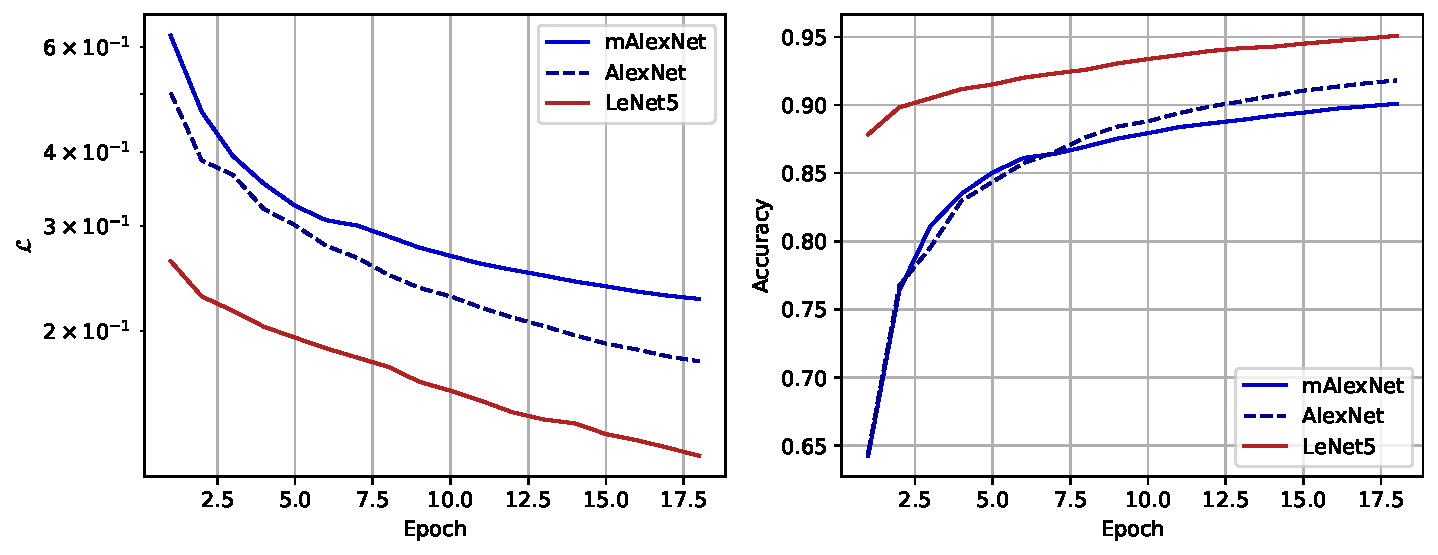
\includegraphics[width=\textwidth]{figures/metrics/loss_acc.pdf}
    \caption{Loss et Accuracy d'AlexNet, mAlexNet and LeNet5 entraînées sur CNRParkEven sur le jeu de données CNRParkOdd.}
    \label{fig:networks_loss_acc}
\end{figure}

Lorsque l'on regarde les statistiques plus avancées en Fig.~\ref{fig:networks_confusion_mat} (une valeur de -1 correspond à un dénominateur nul dans les formules), on peut noter encore une fois la proximité de comportement d'AlexNet et mAlexNet et les meilleurs résultats de LeNet5. On remarque globalement que les métriques concernant les places vides (TNR et NPV) sont toujours inférieures à leurs contreparties "places pleines" (TPR et PPV). Il semble donc plus difficile pour le réseau de prédire qu'une image de place de parking est vide sachant que la place est vide (TNR) que de prédire qu'une image de parking est occupée sachant qu'elle est occupée (TPR).

\begin{figure}[htbp]
    \centering
    \begin{subfigure}{\textwidth}
        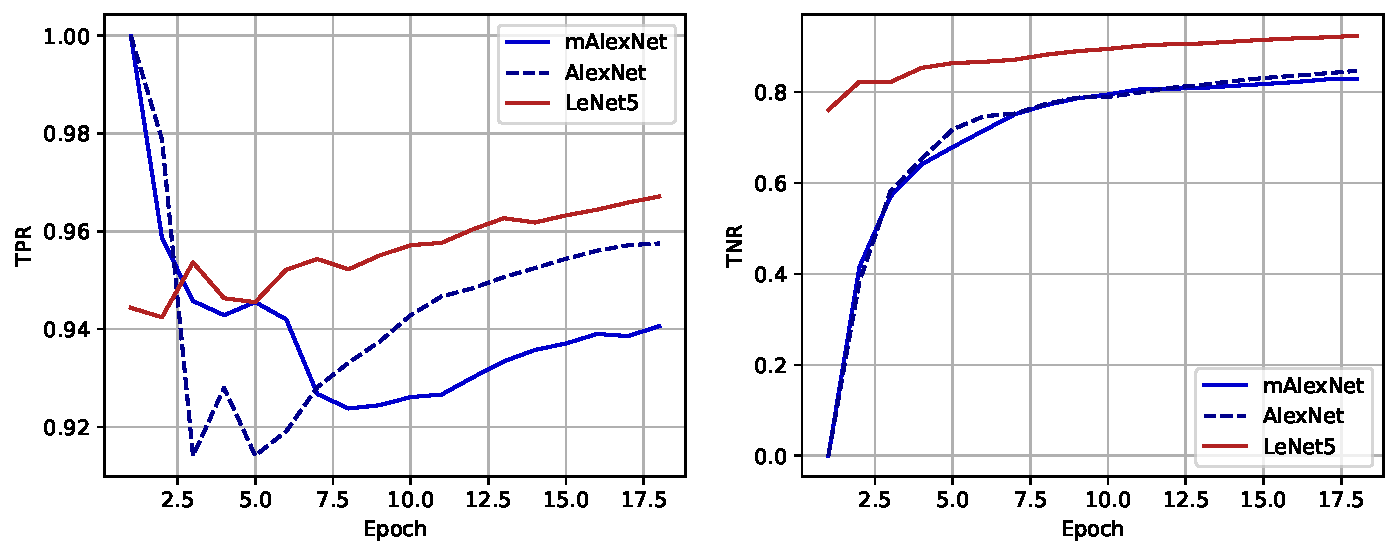
\includegraphics[width=\textwidth]{figures/metrics/true_rates.pdf}
        \caption{TPR et TNR}
    \end{subfigure}
    \begin{subfigure}{\textwidth}
        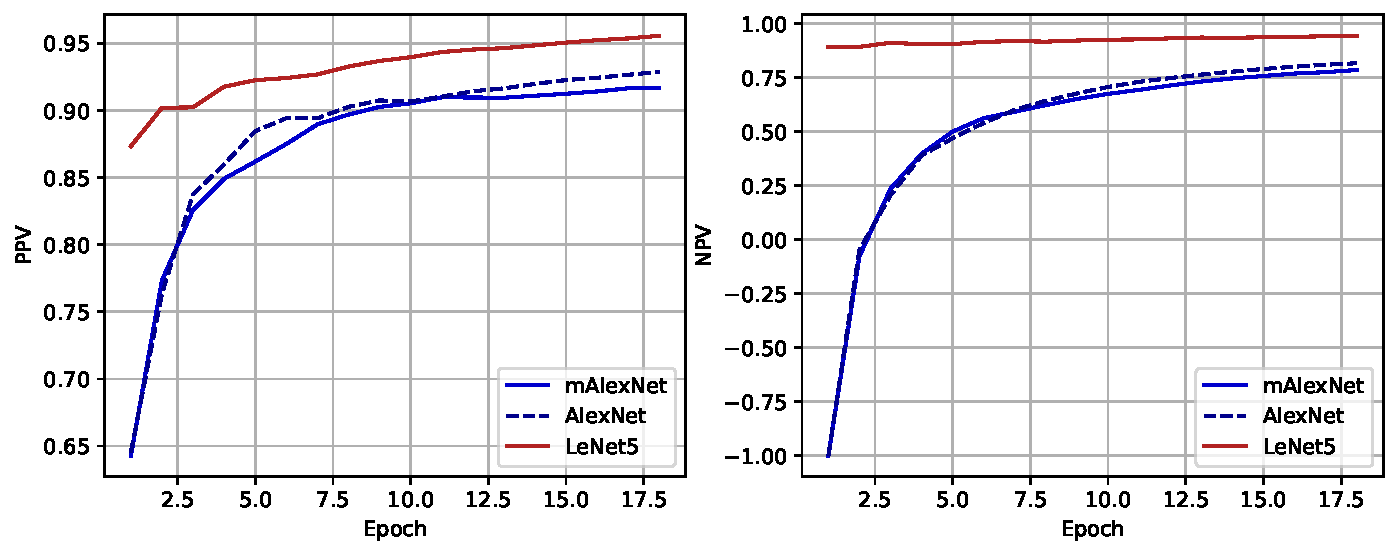
\includegraphics[width=\textwidth]{figures/metrics/predictive_values.pdf}
        \caption{PPV et NPV}
    \end{subfigure}
    \caption{Métriques plus avancées d'AlexNet, mAlexNet and LeNet5 entraînées sur CNRParkEven sur le jeu de données CNRParkOdd.}
    \label{fig:networks_confusion_mat}
\end{figure}

L'exactitude ainsi que les différents métriques avancées des trois réseaux pour les paramètres produisant la meilleure exactitude sur les données de validation sont montrées en Tab.~\ref{tab:results_acc}. On peut remarquer qu'AlexNet et LeNet5 ont une exactitude similaire (91.6\% et 91.5\% respectivement). Les métriques conditionnées révèlent cependant des différences de comportement: le taux de vrais positifs d'AlexNet est supérieure à celui de LeNet5 tandis que le taux de vrais négatifs de LeNet5 est supérieure à celui d'AlexNet.

\begin{table}[htbp]
    \centering
    \begin{tabular}{c | c | c | c | c | c}
        Network & ACC & TPR & TNR & PPV & NPV \\
        \hline
        mAlexNet & 0.897 &      0.949 &      0.780 &      0.906 &      0.873 \\
        AlexNet & 0.916 &      0.960 &      0.818 &      0.922 &      0.902 \\
        LeNet5 & 0.915 &      0.940 &      0.857 &      0.936 &      0.865
    \end{tabular}
    \caption{Métriques sur le jeu de données de test CNRParkOdd d'AlexNet, mAlexNet et LeNet5}
    \label{tab:results_acc}
\end{table}

\section{Optimisation}

Une fois le modèle développé et mis en production, on constate que ses performances sont moins bonnes que lors des tests effectués pendant sa phase de développement. Le principal facteur identifié est que les voitures blanches ne sont pas (ou mal) détectées lorsque le parking est recouvert de neige.

La principale cause de ce défaut est l'absence d'images similaires dans le jeu de données d'entraînement qui n'est pas assez représentatif de la réalité. C'est la raison pour laquelle un nouveau jeu de données CNRPark-EXT est introduit dans le papier \citep{Amato2017} car le jeu de données PKLot \citep{deAlmeida2015} manque d'images de situations difficiles qui peuvent être rencontrées en réalité comme des occlusions et ombrages montrées en Fig.~\ref{fig:cnrpark_ext}. Il faut donc rajouter dans le jeu de données d'entraînement des images de places de parking enneigées.

\begin{figure}[htbp]
    \centering
    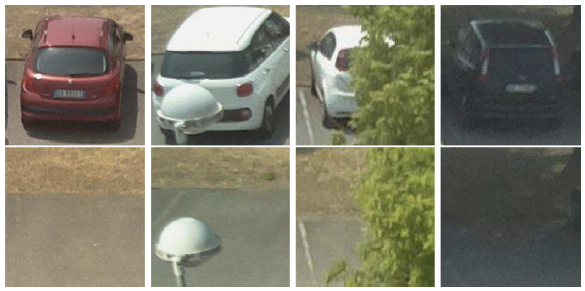
\includegraphics[width=0.8\textwidth]{figures/datasets/cnrpark_ext.png}
    \caption{Des images du jeu de données CNRPark-EXT provenant de \cite{Amato2017}.}
    \label{fig:cnrpark_ext}
\end{figure}

Cette question soulève le problème de la représentativité des données d'entraînement et de leur qualité pour entraîner un réseau de neurones. Dans \cite{Amato2017}, la comparaison des performances des mêmes réseaux entraînés et testés sur différents jeu de données est reproduite en Fig.~\ref{fig:amato2017_results}. Bien que le jeu de données CNRPark est petit (12 000 images) par rapport à PKLot TRAIN (plus de 40 000 images), l'exactitude sur le jeu de données CNRPark-EXT TEST est meilleure en entraînant sur CNRPark pour AlexNet et mAlexNet. Cela montre qu'il faut être vraiment soucieux de la représentativité et de la qualité du jeu de données d'entraînement.

\begin{figure}[htbp]
    \centering
    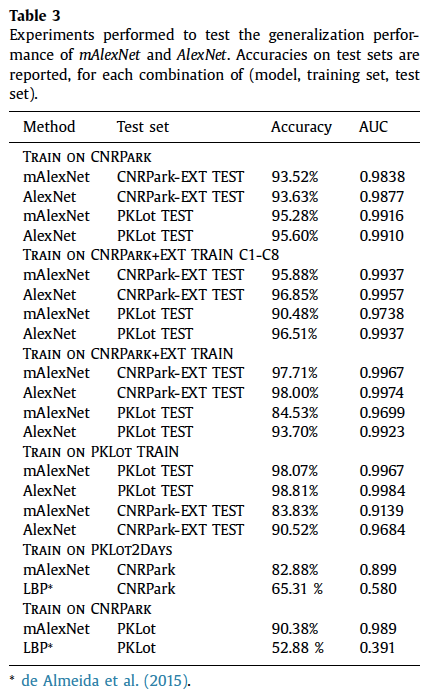
\includegraphics[width=0.4\textwidth]{figures/networks/amato2017_results.png}
    \caption{Résultats d'entraînement de différents CNNs provenant de \cite{Amato2017}.}
    \label{fig:amato2017_results}
\end{figure}

\section{Interprétabilité}

Quantmetry a rejoint le collectif français Confiance.ai lancé par l'Etat dans
le cadre du Grand Défi ”Sécuriser, certifier et fiabiliser les systèmes fondés
sur l'intelligence artificielle”. A ce titre, l'interprétabilité des modèles est une problématique de l'IA (et a fortiori de la Computer Vision) que Quantmetry
propose de résoudre pour ses clients.

Bien que les réseaux de neurones profonds ont montré des résultats impressionants sur de nombreuses tâches, leur interprétabilité est complexe en raison du très grand nombre de paramètres en jeu. Dans de nombreux cas, ces réseaux sont utilisés comme des boîtes noires ce qui peut engendrer beaucoup de risque. L'interprétabilité n'est pas un concept monolithique et englobe plusieurs aspects définis dans \cite{Chakraborty2017}:

\begin{itemize}
    \item La transparence du modèle: cet aspect comprend la reproductibilité du modèle, sa décomposabilité (est ce qu'il y a une explication intuitive des paramètres ?) et enfin sa transparence algorithmique (une manière d'expliquer comment il apprend)
    \item La fonctionnalité du modèle: la sortie du modèle est-elle explicable en quelques phrases ? Peut-on visualiser simplement ses paramètres ? Quels sont les paramètres critiques pour la variabilité du modèle ?
\end{itemize}

Ces dernières années, de nombreuses méthodes pour expliquer ce qui se passe à l'intérieur d'un CNN ont été développé \cite{zhang2018}. Plusieurs approches sont ainsi possibles:

\begin{itemize}
    \item Visualiser les représentations intermédiaires du CNN à travers ses couches intermédiaires et les poids des kernels de convolution
    \item Diagnostic des représentations: trouver une explication sémantique à chaque couche utilisée ou encore extraire des zones d'images qui contributent le plus à la sortie du réseau
    \item Désintriquer les représentations de CNNs en créant des représentations en graphes des zones que le réseau "regarde".
\end{itemize}

\clearpage

\bibliographystyle{unsrtnat}
\setcitestyle{square} %round for parentheses
\bibliography{refs}

\end{document}